\documentclass[10pt,a4paper]{article}
\usepackage[T1]{fontenc}
\usepackage[utf8]{inputenc}
\usepackage{enumitem}
\usepackage{graphicx}
\usepackage{tabularx}
\usepackage{ltablex}
\usepackage{multirow}
\usepackage{helvet}
\usepackage{hhline}
\usepackage{verbatim}
\usepackage[hidelinks]{hyperref}
\usepackage[a4paper,margin=1in]{geometry}
\usepackage{float}
\usepackage[polish]{babel}

\renewcommand\familydefault{\sfdefault}

\begin{document}
\begin{titlepage}
	\centering
	{\Large Wydział Matematyki i Nauk Informacyjnych Politechniki Warszawskiej \par}
	\vspace{1cm}
	
\includegraphics[width=0.2\textwidth]{Resources/Images/logo.png} \par
	\vspace{5cm}
	{\LARGE Aplikacja przeznaczona dla osób\\oglądających seriale telewizyjne \par}
	\vspace{0.5cm}
	{\Large Jacek Dziwulski, Tymon Felski \par}
	\vspace{1.5cm}
	{\Large \today \par}
\end{titlepage}

\newpage
\tableofcontents

\newpage
\section{Raport}

\subsection{Opis logiki aplikacji}
Stworzona w ramach projektu aplikacja \textbf{TV Tracker} jest narzędziem skierowanym do osób regularnie oglądających seriale telewizyjne. Jej celem jest zarówno umożliwienie śledzenia ulubionych programów, jak i odkrywanie nowych, ponieważ na podstawie polubionych seriali, aplikacja proponuje odbiorcy nowe, podobne do nich.\\[\baselineskip]
Użytkownik może się zalogować przy pomocy konta założonego na portalu \textbf{Facebook} lub swoim kontem \textbf{Google}. Przy pierwszym logowaniu zostanie utworzone konto, które będzie odpowiadać za gromadzenie informacji o serialach użytkownika.\\[\baselineskip]
Ekran główny aplikacji zawiera karty z nadchodzącymi odcinkami polubionych seriali. Pod zdjęciem użytkownik znajdzie krótki opis fabuły, niezdradzający zbyt wielu szczegółów, a także opcje pozwalające na przejście do opisu całego serialu lub wyszukanie zwiastunu odcinka w serwisie \textbf{YouTube}.
\begin{figure}[H]
	\centering
	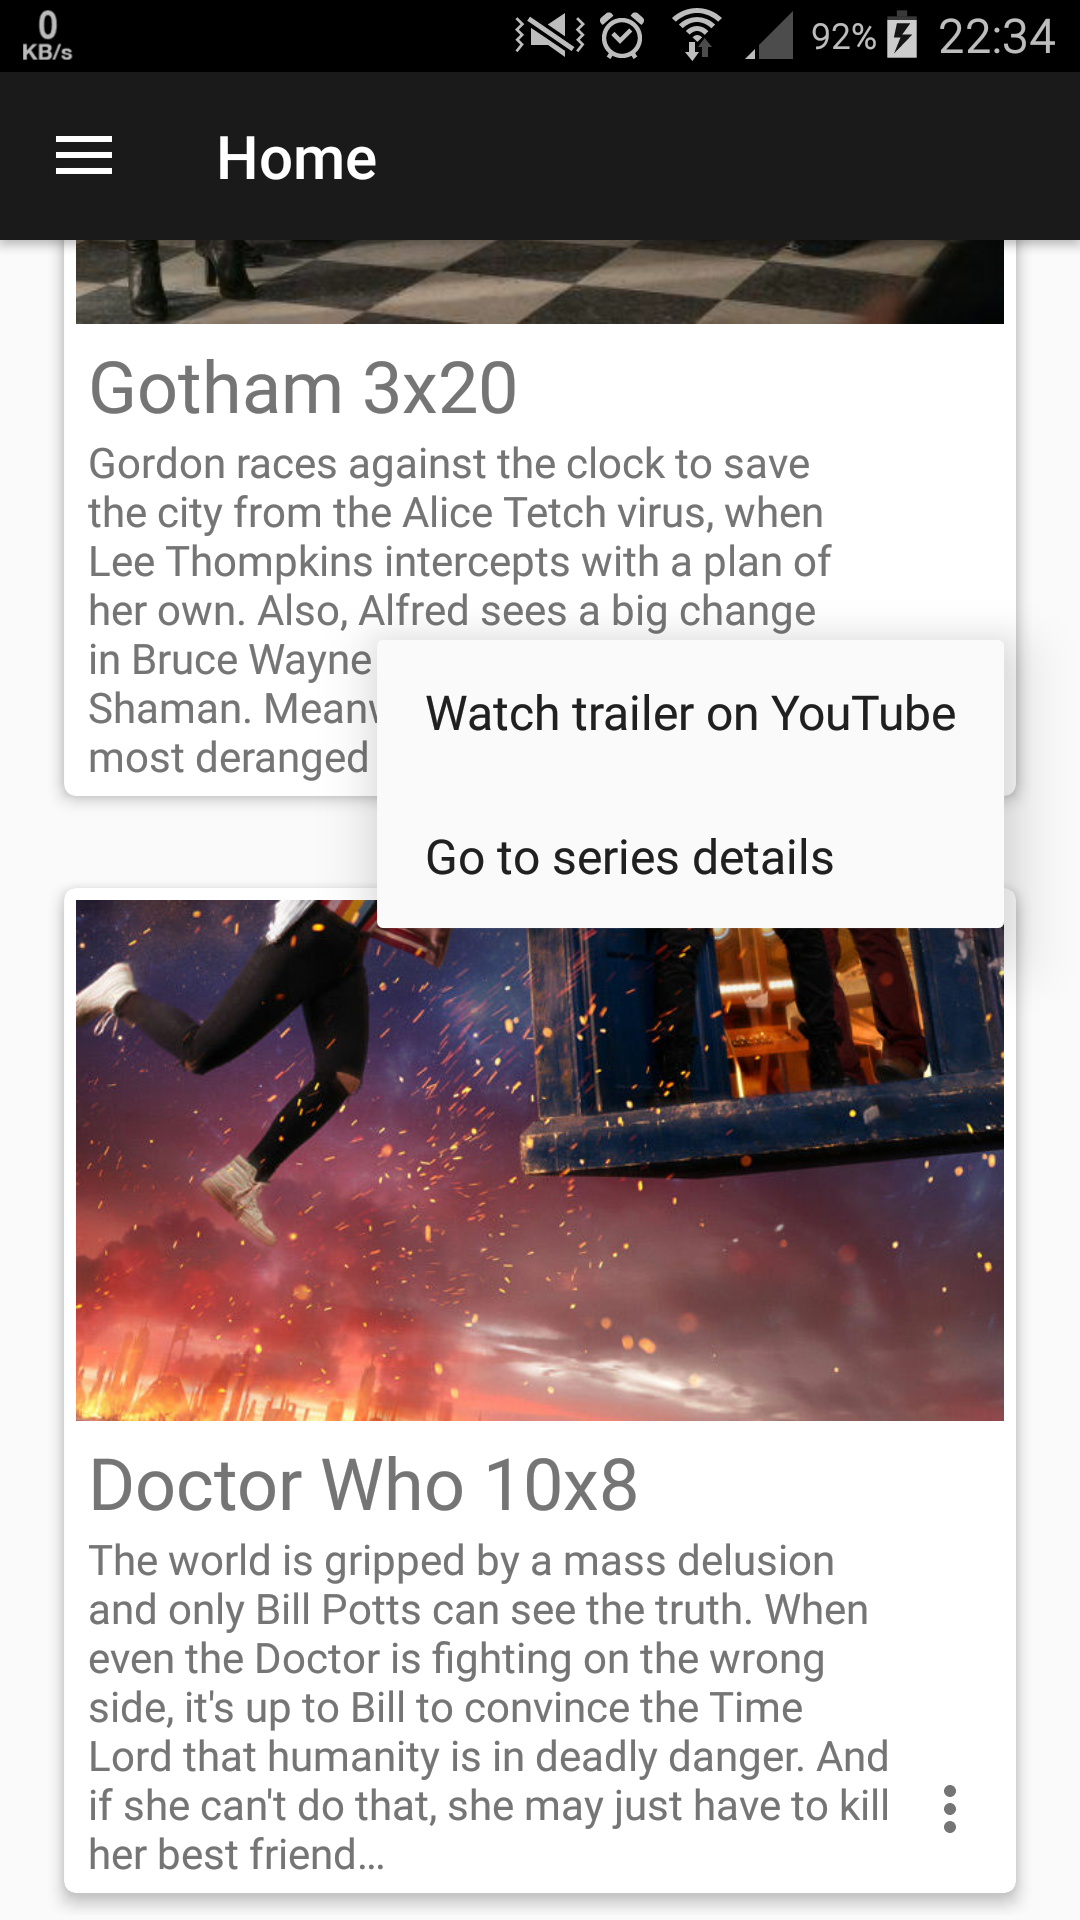
\includegraphics[height=14cm]{Resources/Images/home.png}
	\caption{Ekran główny}
\end{figure}
\newpage
\noindent
Nawigacja w aplikacji odbywa się za pomocą panelu bocznego, w którym poza wszystkimi zakładkami znajdzemy także informacje o zalogowanym użytkowniku - jego zdjęcie, imię i nazwisko oraz adres email. Wybranie jednej z zakładek spowoduje zmianę widoku poprzez podmianę fragmentu.
\begin{figure}[H]
	\centering
	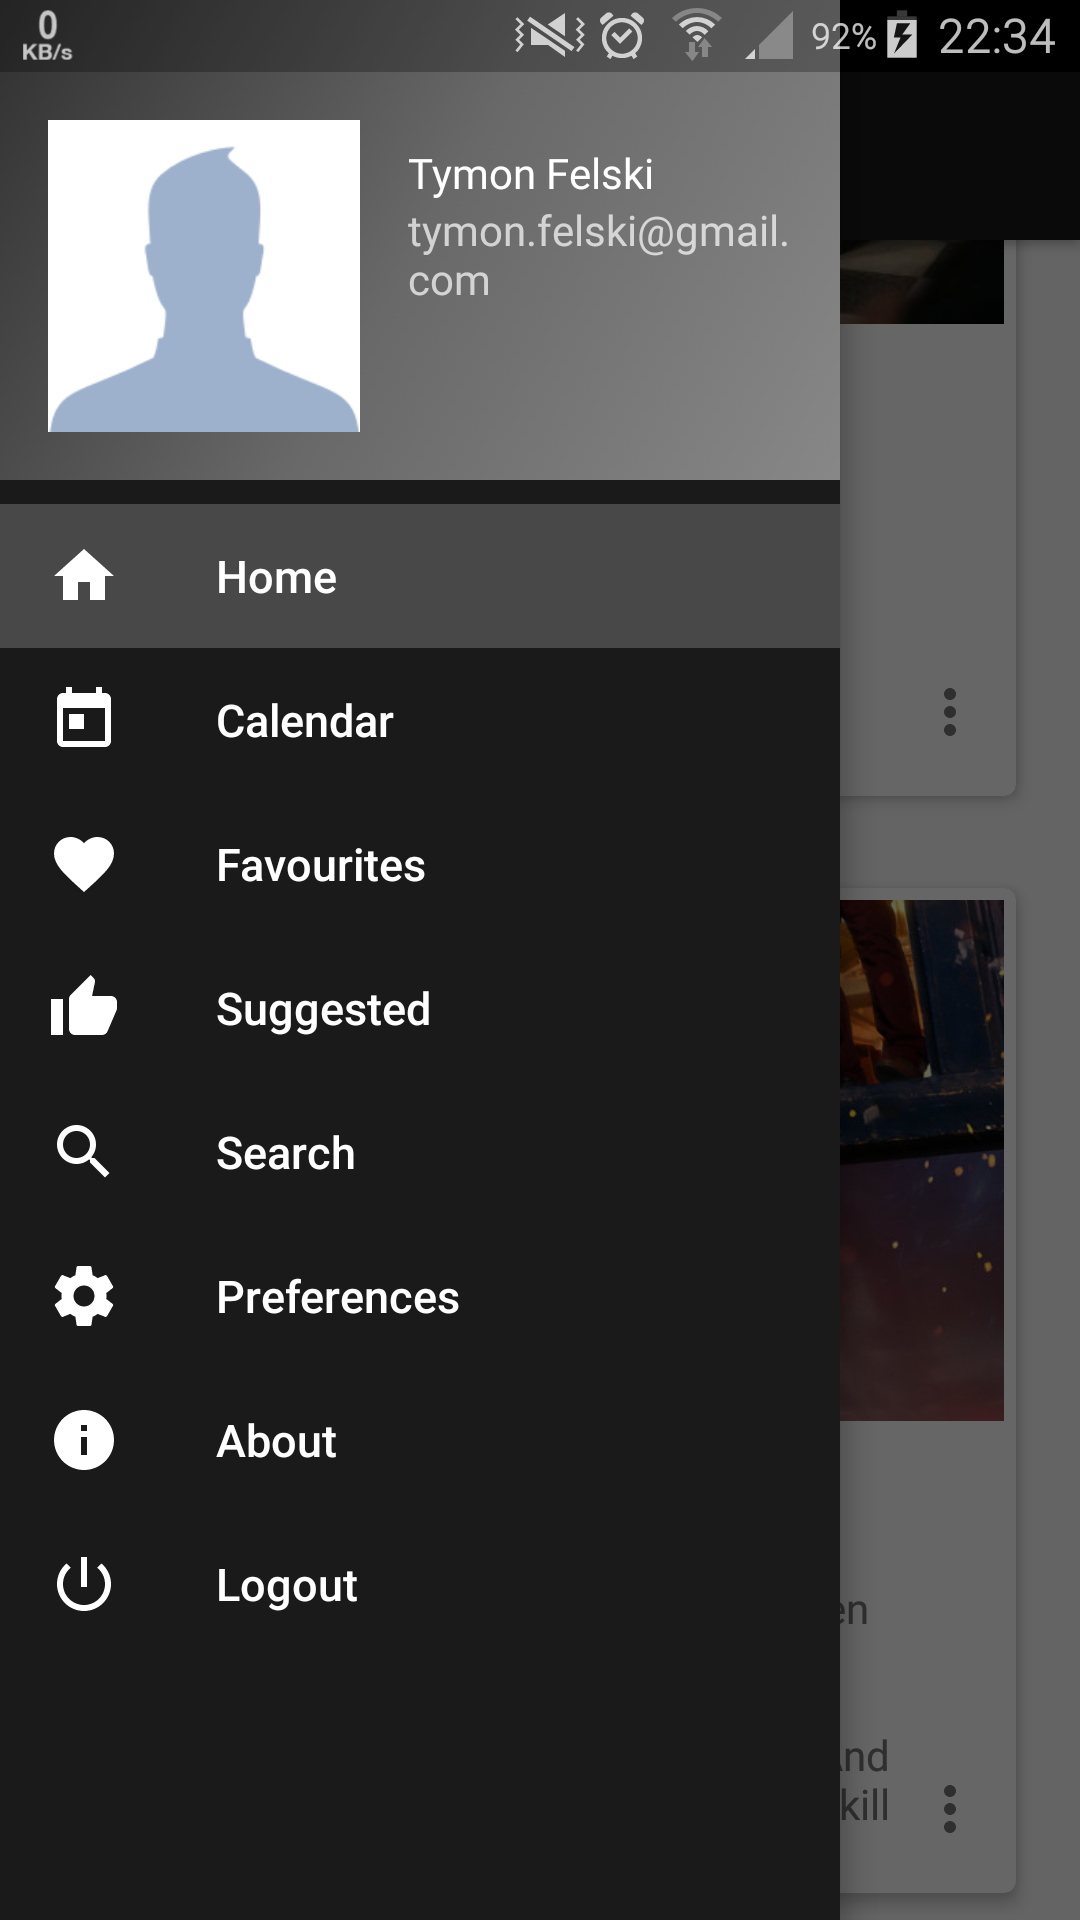
\includegraphics[height=14cm]{Resources/Images/drawer.png}
	\caption{Panel boczny}
\end{figure}
\noindent
Aby znaleźć nowe seriale, należy wejść w zakładkę \textbf{Suggested}, w której pojawi się dwadzieścia seriali najlepiej pasujących do obecnie polubionych lub losowe, jeżeli użytkownik nie dodał żadnych do ulubionych. Można także skorzystać z zakładki \textbf{Search}, gdzie po wpisaniu w pole tekstowe przynajmniej trzech znaków pojawią się seriale spełniające kryteria wyszukiwania.\\[\baselineskip]
Ustawienia aplikacji przewidują możliwość ograniczenia transferu danych w jej obrębie poprzez wyłączenie pobierania obrazków lub zastrzeżenie, że mogą być one pobieranie tylko przy pomocy Wi-Fi.
\newpage
\noindent
Zakładka \textbf{Favourites} zawiera polubione przez użytkownika seriale. Można je stąd usunąć lub wejść w dokładny opis jednego z nich, w którym znajdziemy także wszystkie dotychczasowe odcinki. Użytkownik ma możliwość zaznaczania obejrzanych odcinków. Możliwe jest także wyświetlenie dokładnego opisu danego odcinka poprzez kliknięcie w kartę na ekranie głównym lub przytrzymanie nazwy odcinka na wcześniej wspomnianej liście w opisie serialu.
\begin{figure}[H]
	\centering
	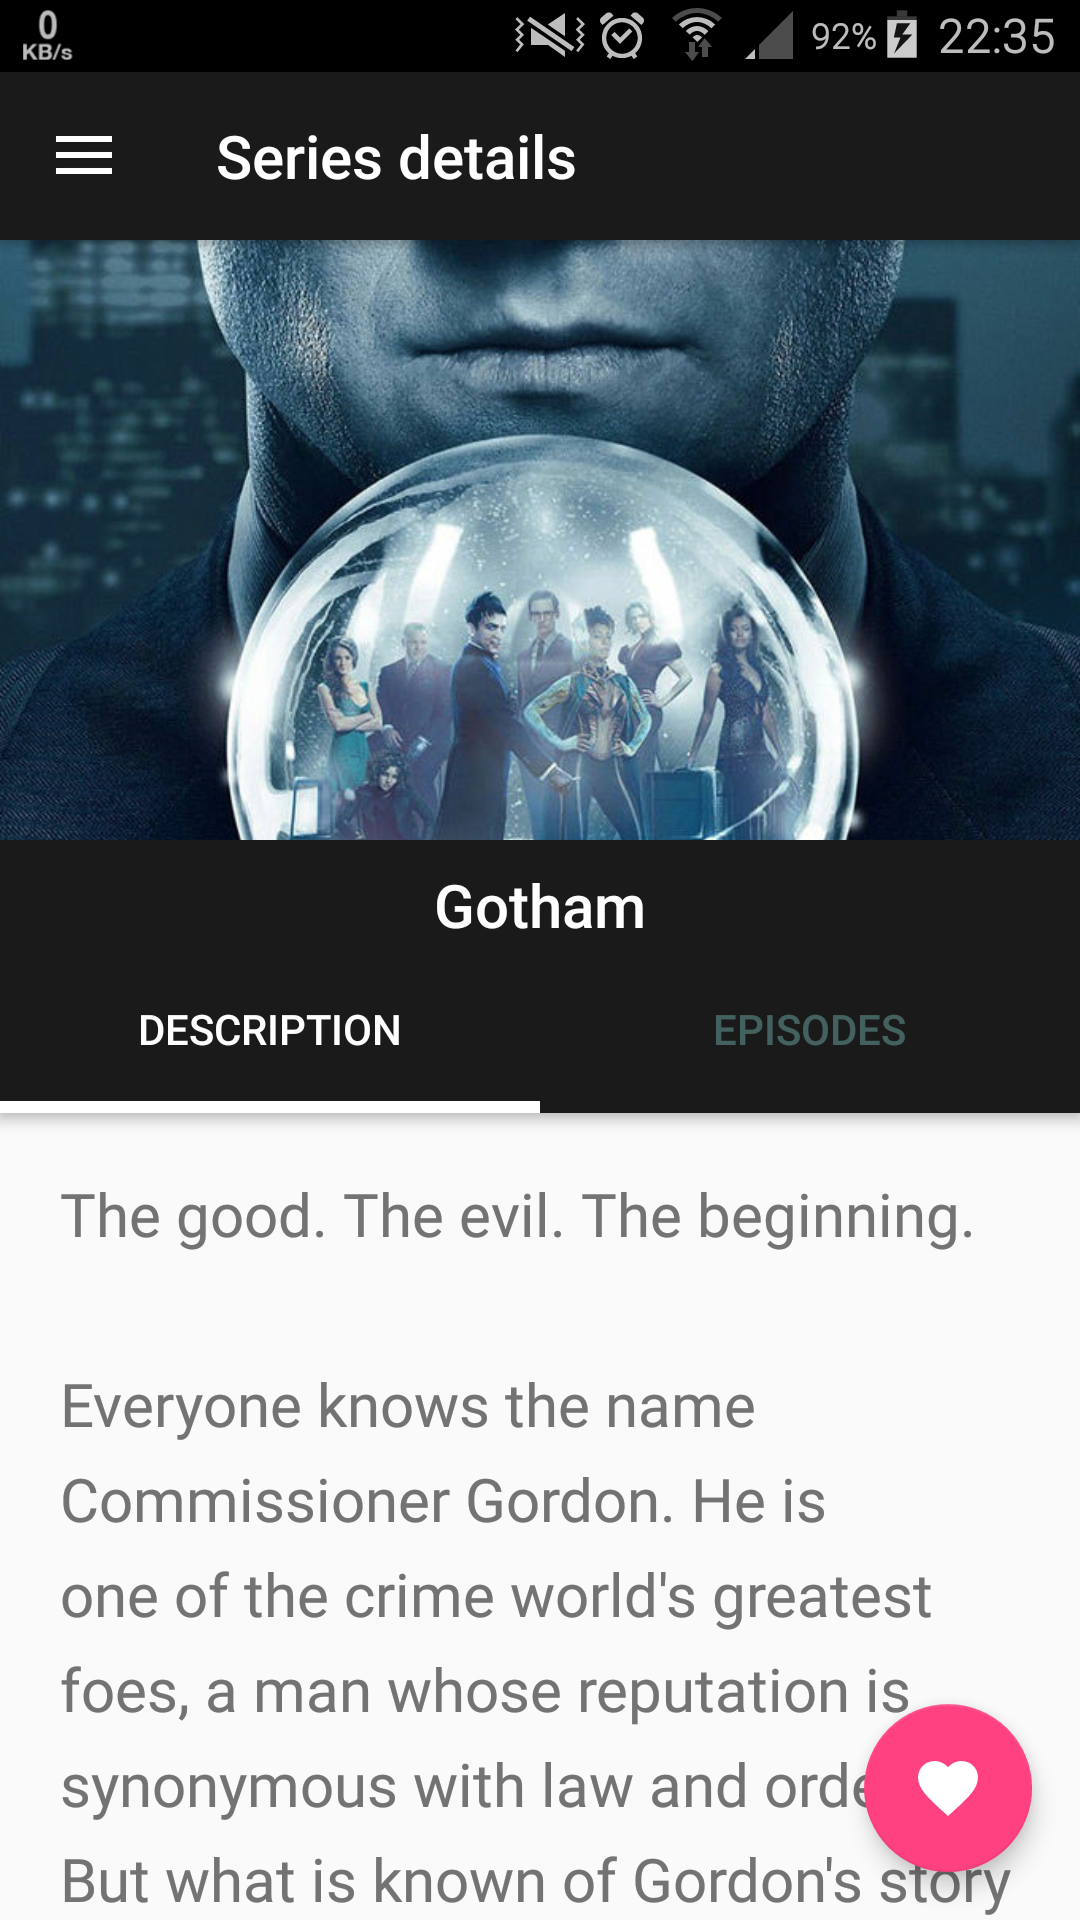
\includegraphics[height=14cm]{Resources/Images/details.png}
	\caption{Opis serialu}
\end{figure}
\noindent
W aplikacji znajduje się także kalendarz, w którym można znaleźć wszystkie odcinki z polubionych seriali. Aplikacja wyśle użytkownikowi powiadomienie przypominające o nadchodzącym odcinku nie później niż pół godziny przed jego rozpoczęciem.

\newpage
\subsection{Opis logiki biznesowej}
Logika biznesowa

\subsubsection{Wykorzystane API}
API

\subsubsection{Serwer .NET WebAPI}
Serwer

\subsection{Wykorzystane rozwiązania}
Wstęp do rozwiązań

\subsubsection{Biblioteki wraz z określeniem licencji}
Przy tworzeniu projektu zostały użyte następujące biblioteki:

\begin{table}[H]
	\begin{tabularx}{\textwidth}{|r|l|X|l|c|}
		\hline
		\textbf{Nr} & \textbf{Komponent i wersja} & \textbf{Opis} & \textbf{Licencja} & \\
		\hline
		1 & 
		Biblioteka, Wersja &
		Opis wykorzystanej biblioteki. &
		\mbox{\hyperref[abbr:lic]{LIC}} &
		\cite{bib} \\
		\hline
	\end{tabularx}
\end{table}

\subsubsection{Wzorce projektowe}
Wzorce

\newpage
\section{Lista użytych skrótów}
\label{abbr:lic}
\paragraph{LIC} LICENSE

\renewcommand*{\refname}{\vspace*{-2em}}
\section{Bibliografia}
\begin{thebibliography}{99}
	\bibitem{bib}
		Biblioteka,
		\emph{Wydawca},
		\url{https://www.biblioteka.com}
\end{thebibliography}

\end{document}
